\originalchapter{作业一：概率密度与涨落}
\psource{8.044，2013 春，PS1，原截止日期 2 月 13 日。以下题面为中文重述；解答为据官方答案核对的 AI 独立推导，纠错处明确注明。}
\originalsection{1．半导体掺杂}
\begin{exercise}
杂质到表面的深度 $x$ 服从 $p(x)=0.8e^{-x/l}/l+0.2\delta(x-d)$（$x\ge0$，其他处为零），$l,d>0$ 为长度；晶界俘获了 20\% 的杂质。(a) 画累计分布，标明关键特征，无须解析式；(b) 求均值；(c) 求方差；(d) 杂质对微波表面阻抗的贡献随深度按 $e^{-x/s}$ 衰减，趋肤深度 $s>0$，求其平均值。
\end{exercise}
\begin{solution}
(a) $F(x)=0$（$x<0$），$F(x)=0.8(1-e^{-x/l})+0.2\Theta(x-d)$（$x\ge0$）；$d$ 处跳跃 $0.2$，两侧斜率为正且递减，极限为 1。(b) 指数部分的一阶矩为 $l$，故 $\avg{x}=0.8l+0.2d$。(c) $\avg{x^2}=1.6l^2+0.2d^2$，所以
\[\Var x=0.96l^2-0.32ld+0.16d^2=0.8l^2+0.16(l-d)^2.\]
原官方答案末行把 $d^2$ 系数印成负号；上式由前一行相减得出，并满足方差非负。(d) 拉普拉斯积分给 $\avg{e^{-x/s}}=0.8/(1+l/s)+0.2e^{-d/s}$；$s\to\infty$ 趋于 1。
\end{solution}
\begin{center}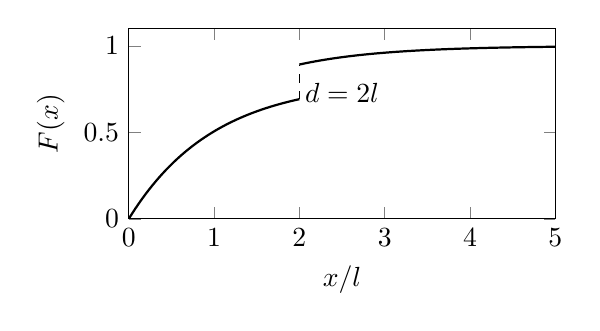
\begin{tikzpicture}\begin{axis}[width=7cm,height=4cm,xmin=0,xmax=5,ymin=0,ymax=1.1,xlabel={$x/l$},ylabel={$F(x)$},samples=80]
\addplot[domain=0:2,thick]{0.8*(1-exp(-x))};\addplot[domain=2:5,thick]{0.8*(1-exp(-x))+0.2};\draw[dashed] (axis cs:2,0.6917)--(axis cs:2,0.8917);\node at(axis cs:2.5,.73){$d=2l$};\end{axis}\end{tikzpicture}\end{center}
\originalsection{2．洛伦兹分布}
\begin{exercise}
$p(x)=a/(b^2+x^2)$，$x\in\mathbb R$，$b>0$；此柯西分布常近似共振谱线。(a) 归一化求 $a$；(b) 求累计分布并画图；(c) 求均值；(d) 求密度降为峰值一半的位置及半高半宽；(e) 讨论二阶矩与方差。
\end{exercise}
\begin{solution}
(a) $\int\dd x/(b^2+x^2)=\pi/b$，故 $a=b/\pi$。(b) $F(x)=1/2+\arctan(x/b)/\pi$，单调 S 形，$F(0)=1/2$，两端极限 0、1。(c) $\int_0^\infty xp(x)\dd x$ 对数发散，负半轴也发散，均值\textbf{不存在}。对称主值为零，不能当作期望；官方答案“由对称性均值零”需纠正。(d) 半高点 $\pm b$，半高半宽 $b$，全宽 $2b$。(e) 二阶矩发散，方差无有限定义。
\end{solution}
\begin{center}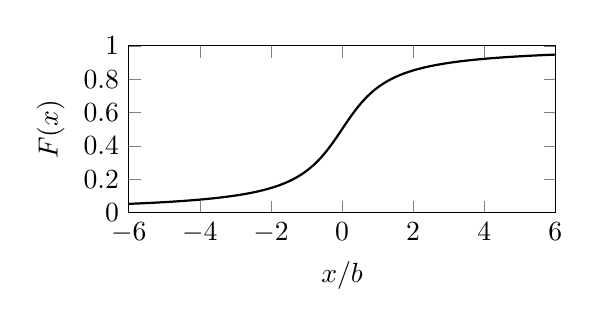
\begin{tikzpicture}\begin{axis}[width=7cm,height=3.7cm,xmin=-6,xmax=6,ymin=0,ymax=1,xlabel={$x/b$},ylabel={$F(x)$},samples=100]\addplot[thick,domain=-6:6]{.5+atan(x)/180};\end{axis}\end{tikzpicture}\end{center}
\originalsection{3．经典振子的可见端点}
\begin{exercise}
将铅笔夹在两指间使它快速摆动，观察两端位置较明显的现象。对 $x=x_0\sin(\omega t+\phi)$，相位完全未知，位置概率正比于在该处停留时间。(a) 求给定 $x$ 的速率；(b) 归一化求 $p(x)$；(c) 画密度，指出最可能、最不可能的可达位置和无需计算的均值，并解释观察。
\end{exercise}
\begin{solution}
(a) $|\dot x|=\omega\sqrt{x_0^2-x^2}$。(b) 每周期两次经过位置元，$p(x)=1/[\pi\sqrt{x_0^2-x^2}]$，$|x|<x_0$，其他处零。(c) 密度在 $\pm x_0$ 可积发散，中心为最低点 $1/(\pi x_0)$，均值零。端点较亮是速率较低、停留较久的结果；固定相位时则为沿轨道移动的 $\delta$ 分布。
\end{solution}
\begin{center}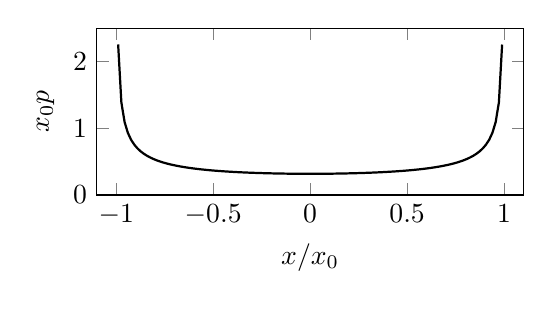
\begin{tikzpicture}\begin{axis}[width=7cm,height=3.7cm,xmin=-1.1,xmax=1.1,ymin=0,ymax=2.5,xlabel={$x/x_0$},ylabel={$x_0p$},samples=120]\addplot[thick,domain=-.99:.99]{1/(pi*sqrt(1-x*x))};\end{axis}\end{tikzpicture}\end{center}
\originalsection{4．量子化角动量}
\begin{exercise}
$L_x$ 只能取 $-\hbar,0,\hbar$，已知 $\avg{L_x}=\hbar/3$、$\avg{L_x^2}=2\hbar^2/3$。(a) 求并画概率密度；(b) 画带标记的累计分布。
\end{exercise}
\begin{solution}
归一化、一阶矩、二阶矩给 $p_-+p_0+p_+=1$、$p_+-p_-=1/3$、$p_++p_-=2/3$，故 $p_-=1/6,p_0=1/3,p_+=1/2$。密度为相应权重的三个 $\delta$ 峰。累计函数在三个位置依次从 0 跳至 $1/6,1/2,1$，取右连续值。下列密度图箭头表示单位面积 $\delta$ 的权重，不是有限峰高。
\end{solution}
\begin{center}\begin{tikzpicture}[x=1.5cm,y=1.8cm]\draw[->](-1.6,0)--(1.7,0)node[right]{$L_x/\hbar$};\draw[->](0,-.1)--(0,1.2)node[above]{$F$};\draw[thick](-1.5,0)--(-1,0) (-1,.1667)--(0,.1667) (0,.5)--(1,.5) (1,1)--(1.5,1);\draw[dashed](-1,0)--(-1,.1667) (0,.1667)--(0,.5) (1,.5)--(1,1);\node[below]at(-1,0){$-1$};\node[below]at(1,0){$1$};\node[left]at(0,.5){$1/2$};\end{tikzpicture}\end{center}
\begin{center}\begin{tikzpicture}[x=1.6cm,y=3cm]\draw[->](-1.5,0)--(1.6,0)node[right]{$L_x/\hbar$};\draw[->](-1,0)--(-1,.1667)node[above]{$1/6$};\draw[->](0,0)--(0,.3333)node[above]{$1/3$};\draw[->](1,0)--(1,.5)node[above]{$1/2$};\node[below]at(-1,0){$-1$};\node[below]at(0,0){$0$};\node[below]at(1,0){$1$};\end{tikzpicture}\end{center}
\originalsection{5．相干态的运动}
\begin{exercise}
一维波函数为
\[\Psi(x,t)=(2\pi x_0^2)^{-1/4}\exp\left[-\frac{i\omega t}{2}-\frac{i(2\alpha xx_0\sin\omega t-\alpha^2x_0^2\sin2\omega t)}{(2x_0)^2}-\left(\frac{x-2\alpha x_0\cos\omega t}{2x_0}\right)^2\right].\]
$x_0$ 是长度，$\alpha$ 无量纲。(a) 求 $p=|\Psi|^2$；(b) 直接读出均值、方差；(c) 简述运动并画 $t=0,T/4,T/2,3T/4,T$ 的密度，$T=2\pi/\omega$。
\end{exercise}
\begin{solution}
纯相位模方为一，$p=\exp[-(x-2\alpha x_0\cos\omega t)^2/(2x_0^2)]/(\sqrt{2\pi}x_0)$。均值 $2\alpha x_0\cos\omega t$，方差 $x_0^2$。高斯不变形地往返；上述五时刻中心依次为 $2\alpha x_0,0,-2\alpha x_0,0,2\alpha x_0$。图取 $\alpha=1$；两个重复时刻曲线重合。
\end{solution}
\begin{center}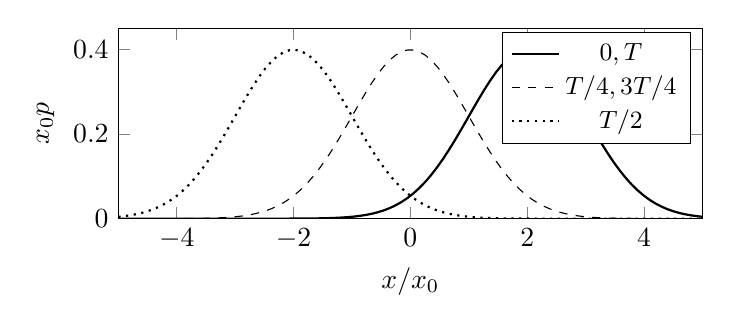
\begin{tikzpicture}\begin{axis}[width=9cm,height=4cm,xmin=-5,xmax=5,ymin=0,ymax=.45,xlabel={$x/x_0$},ylabel={$x_0p$},samples=100,legend style={font=\small}]
\addplot[domain=-5:5,thick]{exp(-(x-2)^2/2)/sqrt(2*pi)};\addlegendentry{$0,T$}
\addplot[domain=-5:5,dashed]{exp(-x*x/2)/sqrt(2*pi)};\addlegendentry{$T/4,3T/4$}
\addplot[domain=-5:5,dotted,thick]{exp(-(x+2)^2/2)/sqrt(2*pi)};\addlegendentry{$T/2$}\end{axis}\end{tikzpicture}\end{center}
\originalsection{6．单模玻色光子数}
\begin{exercise}
腔内一模光子数 $n=0,1,\ldots$ 服从 $p_n=(1-a)a^n$，$0\le a<1$；每光子能量 $\hbar\omega$。(a) 对几何级数求导得平均数；(b) 求方差并以平均数表示，指出比同均值泊松分布大几倍；(c) 将密度写成指数包络乘非负整数处的单位面积 $\delta$ 列，求衰减长度 $\phi$，证明大平均数时 $\phi\sim\avg n$。
\end{exercise}
\begin{solution}
从 $\sum a^n=(1-a)^{-1}$ 用 $a\partial_a$ 一次、两次，得 $\avg n=a/(1-a)$、$\avg{n^2}=2\avg n^2+\avg n$，故 $\Var n=\avg n(1+\avg n)$，增强因子 $1+\avg n$。$p(x)=(1-a)e^{-x/\phi}\sum_{n\ge0}\delta(x-n)$，$\phi=-1/\ln a=1/\ln(1+1/\avg n)$；由 $\ln(1+y)\sim y$ 得极限。$a=0$ 时仅 $n=0$，应直接取退化分布。
\end{solution}
